\subsection{Serial Communication and the Great Horse Race}
The input of the system is handled using MATLAB. This is appealing for several
reasons, (1), we can immedietly visualise and process the sound array that we
get, making it easy to debu, and (2), we can use the inbuilt system microphone.
MATLAB by default offers several different ways to get this audio data, the
lowest resolution being a 1000Hz Sampling frequency and 8-bit sampling, using
the \texttt{audiorecorder} object. Once we record the relevent sample, we
extract an array with this data and after doing some basic filtering, to remove
any high frequency noise that may affect the signal, we send the data to the
Arduino via the Serial port. 

The important part here is understanding how the serial communication with the
Arduino works. The serial port can only send data character by character to the
Arduino and waits for it to be processed. Therefore the processing of the
integers is done as follows: 

\begin{enumerate}
    \item Collect multiple audio samples from the microphone. We take 2000
    datapoints, assuming a periodic sample. The points are all \texttt{int8}.

    \item Apply a filter to remove any peaks above \(\pm7\) to ensure that the
    data doesn't overflow in the arduino. Then we apply a Moving average filter
    by taking 3 200-datapoint samples from the 2000 datapoints to remove any
    anamolous noise in the data.

    \item In order to communicate this data, we convert the integer Array in
    MATLAB to strings using the \texttt{int2str} method so that it can be sent
    via the Serial port. The terminator that we use is the newline character
    '$\backslash$n'.

    \item We open the serial monitor and send the data character by character
    using the \texttt{fprintf} function in Matlab.

    \item We check for available data in the Arduino using the
    \texttt{Serial.available()} function.

    \item Then we read the data into an array in Arduino using the
    \texttt{Serial.parseInt()} function. We wait for 2 bytes to arrive and store
    them in a single byte on the arduino to work with our processing scheme.
    
    \item When all the expected data (200 points) are read, stop recording and
    do the processing to find the matching frequencies. 

    \item Send the frequencies back to MATLAB to print using the Serial port. 
\end{enumerate}
This protocol can be seen in this block diagram 
\begin{figure}[ht]
    \centering
    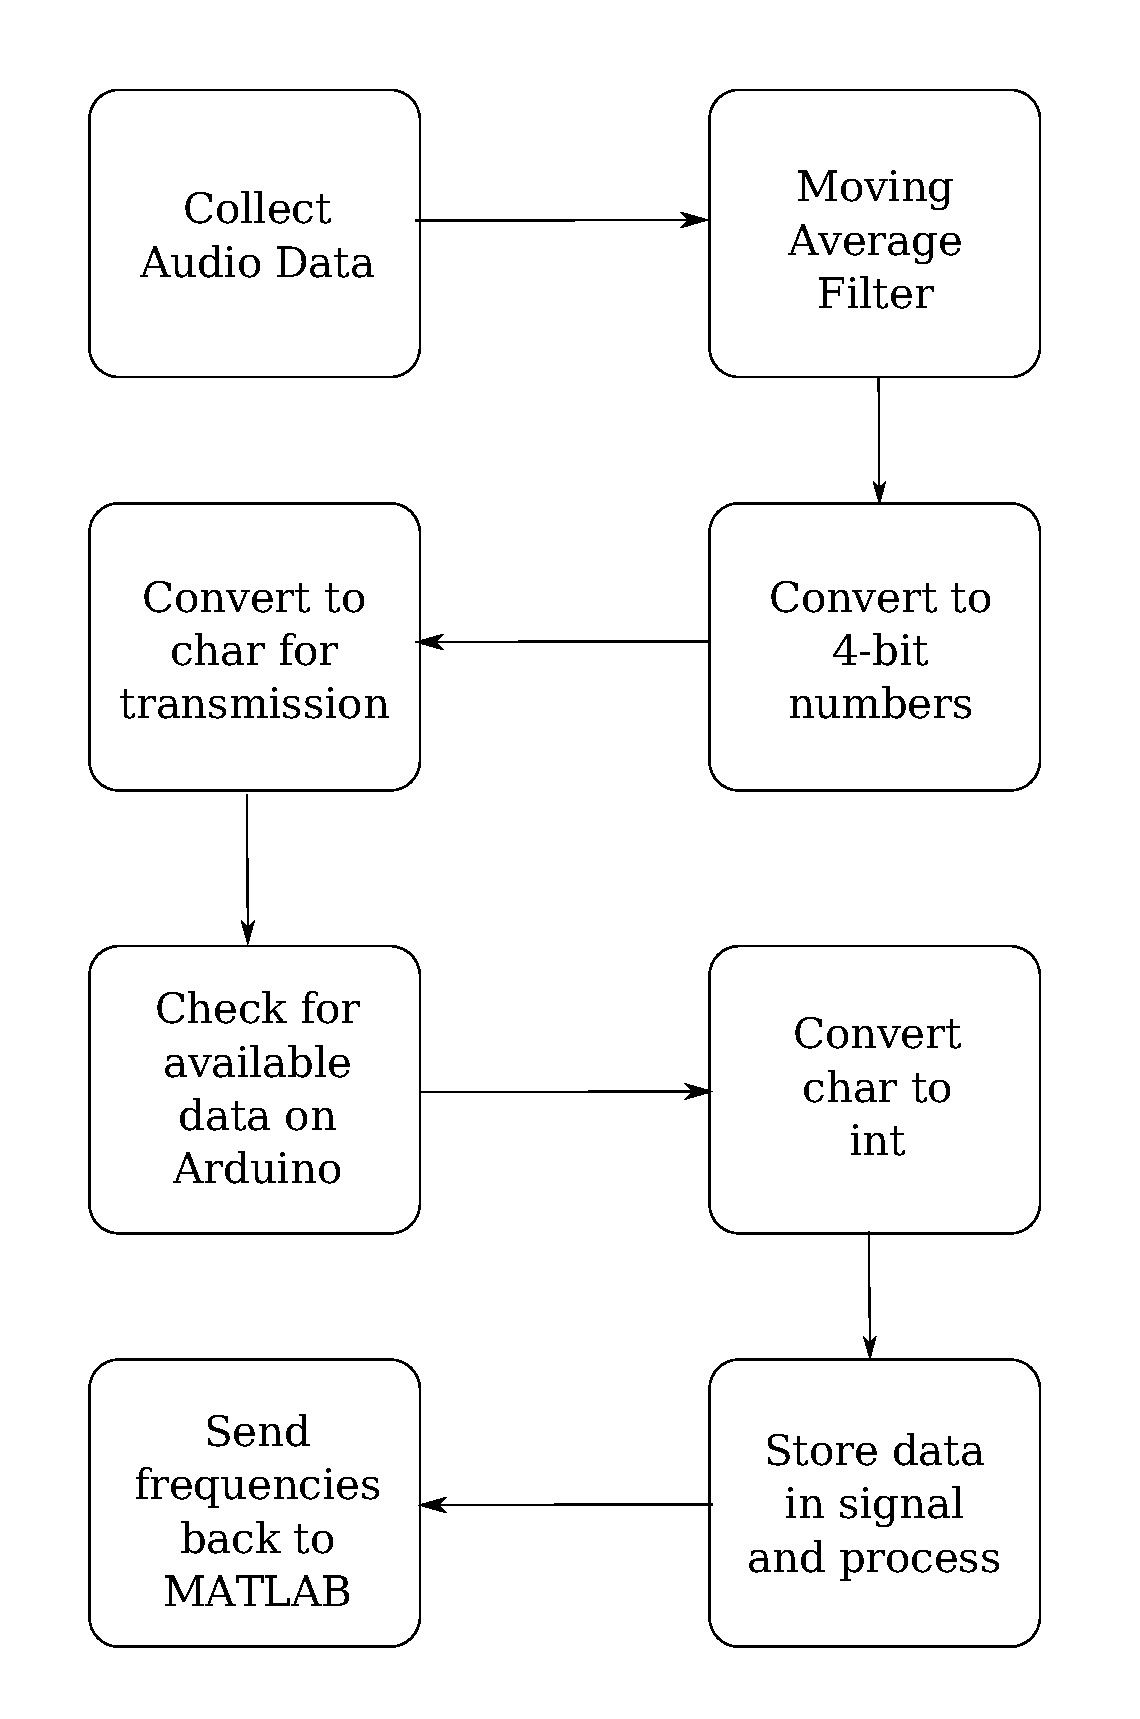
\includegraphics[width=0.6\textwidth]{fig/commsblock.pdf}
    \caption{Block diagram for communication protocol.}
    \label{fig:commsblock}
\end{figure}

However, we ran into some issues here, where several values were not detected by
the Arduino. We tried multiple approaches to solve this 

\begin{enumerate}
    \item We increased the Baud rate to 115200 to ensure that the transmission
    wasn't causing any loss of data. 

    \item We added a small delay of 30ms between subsequent transmissions to
    ensure that the Arduino had time to process the data.

    \item The Serial protocol has a buffer that stores the incoming values
    before they are processed by the Arduino. In the Arduino Uno, this
    \texttt{SERIAL\_RX\_BUFFER} memory that stores the incoming data from the
    Serial Port is only 64 bytes. We changed the header files to make the buffer
    128 bytes in HardwareSerial.h so that more characters could be stored
    without losing them in transmission.
\end{enumerate}

In order to ensure that this method is working correctly we have several checks 

\begin{enumerate}
    \item We ran a simple program that turns the pin13 LED On and Off based on
    whether the character it received was 0 or -7.

    \item In our main code, pin 13 is HIGH when waiting for data and recording.
    When all the expected data has been found, it stops glowing.
    
    \item We also plot the raw data that we get from the Mic to ensure that a
    reasonable waveform has been detected.
\end{enumerate}

The code for testing the glowing of the LEDs is found here: 

\begin{lstlisting}[language=C++]
const int led = 13;
String text;
int k;
void setup() {
                //pinMode(led, OUTPUT);
                Serial.begin(9600);
                k = 0;
}
void loop() { 
  if (Serial.available()){
                    text = Serial.readStringUntil('$');
                    k = text.toInt(); 
                    if(k == -7){
                        digitalWrite(led, 1);
                    }
                    if(k == 0){
                        digitalWrite(led, 0);
                    }
  }
}
\end{lstlisting}

The MATLAB code for controlling this unit is found here: 

\begin{lstlisting}[language=Matlab]
Arduino = serial("COM4","BaudRate",9600);
fopen(Arduino) %This opens a monitor
fprintf(Arduino,'%s$',int2str(0));
fprintf(Arduino,'%s$',int2str(-7));
fclose(Arduino);
\end{lstlisting}

